\documentclass{standalone}
\usepackage{tikz}
\usetikzlibrary{patterns, positioning}


\begin{document}
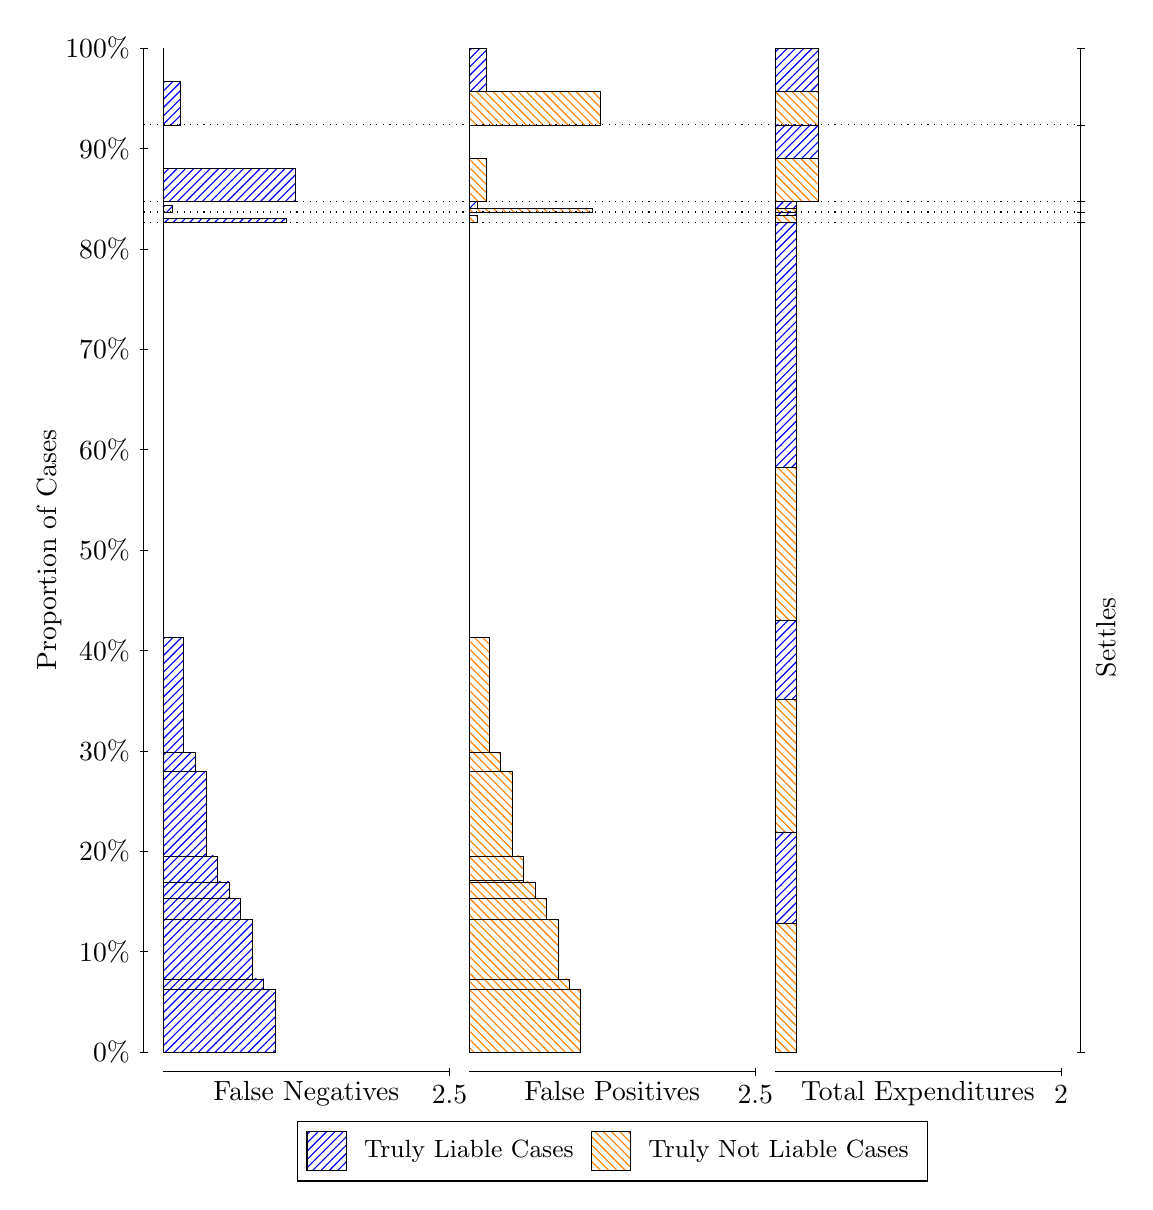
\begin{tikzpicture}
\draw[black, very thin] (1.5,1.75) -- (1.5,14.5);
\node[rotate=90, text=black, anchor=center] at (0.3, 8.125) {Proportion of Cases};
\draw[black, very thin] (1.45,1.75) -- (1.55,1.75);
\node[text=black, anchor=east] at (1.45, 1.75) {0\%};
\draw[black, very thin] (1.45,3.025) -- (1.55,3.025);
\node[text=black, anchor=east] at (1.45, 3.025) {10\%};
\draw[black, very thin] (1.45,4.3) -- (1.55,4.3);
\node[text=black, anchor=east] at (1.45, 4.3) {20\%};
\draw[black, very thin] (1.45,5.575) -- (1.55,5.575);
\node[text=black, anchor=east] at (1.45, 5.575) {30\%};
\draw[black, very thin] (1.45,6.85) -- (1.55,6.85);
\node[text=black, anchor=east] at (1.45, 6.85) {40\%};
\draw[black, very thin] (1.45,8.125) -- (1.55,8.125);
\node[text=black, anchor=east] at (1.45, 8.125) {50\%};
\draw[black, very thin] (1.45,9.4) -- (1.55,9.4);
\node[text=black, anchor=east] at (1.45, 9.4) {60\%};
\draw[black, very thin] (1.45,10.675) -- (1.55,10.675);
\node[text=black, anchor=east] at (1.45, 10.675) {70\%};
\draw[black, very thin] (1.45,11.95) -- (1.55,11.95);
\node[text=black, anchor=east] at (1.45, 11.95) {80\%};
\draw[black, very thin] (1.45,13.225) -- (1.55,13.225);
\node[text=black, anchor=east] at (1.45, 13.225) {90\%};
\draw[black, very thin] (1.45,14.5) -- (1.55,14.5);
\node[text=black, anchor=east] at (1.45, 14.5) {100\%};

\draw[black, very thin] (13.4,1.75) -- (13.4,14.5);
\draw[black, very thin] (13.35,1.75) -- (13.45,1.75);
\node[anchor=west] at (13.35, 1.75) {};
\draw[black, very thin] (13.35,12.286) -- (13.45,12.286);
\node[anchor=west] at (13.35, 12.286) {};
\draw[black, very thin] (13.35,12.418) -- (13.45,12.418);
\node[anchor=west] at (13.35, 12.418) {};
\draw[black, very thin] (13.35,12.549) -- (13.45,12.549);
\node[anchor=west] at (13.35, 12.549) {};
\draw[black, very thin] (13.35,13.525) -- (13.45,13.525);
\node[anchor=west] at (13.35, 13.525) {};
\draw[black, very thin] (13.35,14.5) -- (13.45,14.5);
\node[anchor=west] at (13.35, 14.5) {};

\draw[black, very thin, pattern color=blue, pattern=north east lines] (1.75,1.75) rectangle (3.167,2.5442);
\draw[black, very thin, pattern color=blue, pattern=north east lines] (1.75,2.5442) rectangle (3.0217,2.6794);
\draw[black, very thin, pattern color=blue, pattern=north east lines] (1.75,2.6794) rectangle (2.8763,3.4361);
\draw[black, very thin, pattern color=blue, pattern=north east lines] (1.75,3.4361) rectangle (2.731,3.7011);
\draw[black, very thin, pattern color=blue, pattern=north east lines] (1.75,3.7011) rectangle (2.5857,3.9106);
\draw[black, very thin, pattern color=blue, pattern=north east lines] (1.75,3.9106) rectangle (2.4403,4.2393);
\draw[black, very thin, pattern color=blue, pattern=north east lines] (1.75,4.2393) rectangle (2.295,5.3164);
\draw[black, very thin, pattern color=blue, pattern=north east lines] (1.75,5.3164) rectangle (2.1497,5.55);
\draw[black, very thin, pattern color=blue, pattern=north east lines] (1.75,5.55) rectangle (2.0043,7.0178);
\draw[black, very thin, pattern color=orange, pattern=north west lines] (1.75,7.0178) rectangle (1.75,12.286);
\draw[black, very thin, pattern color=blue, pattern=north east lines] (1.75,12.286) rectangle (3.3123,12.332);
\draw[black, very thin, pattern color=orange, pattern=north west lines] (1.75,12.332) rectangle (1.75,12.418);
\draw[black, very thin, pattern color=blue, pattern=north east lines] (1.75,12.418) rectangle (1.859,12.503);
\draw[black, very thin, pattern color=orange, pattern=north west lines] (1.75,12.503) rectangle (1.75,12.549);
\draw[black, very thin, pattern color=blue, pattern=north east lines] (1.75,12.549) rectangle (3.4213,12.976);
\draw[black, very thin, pattern color=orange, pattern=north west lines] (1.75,12.976) rectangle (1.75,13.525);
\draw[black, very thin, pattern color=blue, pattern=north east lines] (1.75,13.525) rectangle (1.968,14.074);
\draw[black, very thin, pattern color=orange, pattern=north west lines] (1.75,14.074) rectangle (1.75,14.5);
\draw[black, very thin, pattern color=orange, pattern=north west lines] (5.6333,1.75) rectangle (7.0503,2.5441);
\draw[black, very thin, pattern color=orange, pattern=north west lines] (5.6333,2.5441) rectangle (6.905,2.6794);
\draw[black, very thin, pattern color=orange, pattern=north west lines] (5.6333,2.6794) rectangle (6.7597,3.4361);
\draw[black, very thin, pattern color=orange, pattern=north west lines] (5.6333,3.4361) rectangle (6.6143,3.7011);
\draw[black, very thin, pattern color=orange, pattern=north west lines] (5.6333,3.7011) rectangle (6.469,3.9106);
\draw[black, very thin, pattern color=orange, pattern=north west lines] (5.6333,3.9106) rectangle (6.3237,3.9263);
\draw[black, very thin, pattern color=orange, pattern=north west lines] (5.6333,3.9263) rectangle (6.3237,4.2392);
\draw[black, very thin, pattern color=orange, pattern=north west lines] (5.6333,4.2392) rectangle (6.1783,5.3164);
\draw[black, very thin, pattern color=orange, pattern=north west lines] (5.6333,5.3164) rectangle (6.033,5.55);
\draw[black, very thin, pattern color=orange, pattern=north west lines] (5.6333,5.55) rectangle (5.8877,7.0178);
\draw[black, very thin, pattern color=blue, pattern=north east lines] (5.6333,7.0178) rectangle (5.6333,12.286);
\draw[black, very thin, pattern color=orange, pattern=north west lines] (5.6333,12.286) rectangle (5.7423,12.371);
\draw[black, very thin, pattern color=blue, pattern=north east lines] (5.6333,12.371) rectangle (5.6333,12.418);
\draw[black, very thin, pattern color=orange, pattern=north west lines] (5.6333,12.418) rectangle (7.1957,12.464);
\draw[black, very thin, pattern color=blue, pattern=north east lines] (5.6333,12.464) rectangle (5.7423,12.549);
\draw[black, very thin, pattern color=orange, pattern=north west lines] (5.6333,12.549) rectangle (5.8513,13.098);
\draw[black, very thin, pattern color=blue, pattern=north east lines] (5.6333,13.098) rectangle (5.6333,13.525);
\draw[black, very thin, pattern color=orange, pattern=north west lines] (5.6333,13.525) rectangle (7.3047,13.951);
\draw[black, very thin, pattern color=blue, pattern=north east lines] (5.6333,13.951) rectangle (5.8513,14.5);
\draw[black, very thin, pattern color=orange, pattern=north west lines] (9.5167,1.75) rectangle (9.7892,3.3894);
\draw[black, very thin, pattern color=blue, pattern=north east lines] (9.5167,3.3894) rectangle (9.7892,4.5464);
\draw[black, very thin, pattern color=orange, pattern=north west lines] (9.5167,4.5464) rectangle (9.7892,6.2237);
\draw[black, very thin, pattern color=blue, pattern=north east lines] (9.5167,6.2237) rectangle (9.7892,7.2274);
\draw[black, very thin, pattern color=orange, pattern=north west lines] (9.5167,7.2274) rectangle (9.7892,9.1785);
\draw[black, very thin, pattern color=blue, pattern=north east lines] (9.5167,9.1785) rectangle (9.7892,12.286);
\draw[black, very thin, pattern color=orange, pattern=north west lines] (9.5167,12.286) rectangle (9.7892,12.371);
\draw[black, very thin, pattern color=blue, pattern=north east lines] (9.5167,12.371) rectangle (9.7892,12.418);
\draw[black, very thin, pattern color=orange, pattern=north west lines] (9.5167,12.418) rectangle (9.7892,12.464);
\draw[black, very thin, pattern color=blue, pattern=north east lines] (9.5167,12.464) rectangle (9.7892,12.549);
\draw[black, very thin, pattern color=orange, pattern=north west lines] (9.5167,12.549) rectangle (10.062,13.098);
\draw[black, very thin, pattern color=blue, pattern=north east lines] (9.5167,13.098) rectangle (10.062,13.525);
\draw[black, very thin, pattern color=orange, pattern=north west lines] (9.5167,13.525) rectangle (10.062,13.951);
\draw[black, very thin, pattern color=blue, pattern=north east lines] (9.5167,13.951) rectangle (10.062,14.5);
\draw[black, dotted] (1.5,12.286) -- (13.4,12.286);
\draw[black, dotted] (1.5,12.418) -- (13.4,12.418);
\draw[black, dotted] (1.5,12.549) -- (13.4,12.549);
\draw[black, dotted] (1.5,13.525) -- (13.4,13.525);
\draw[black, very thin] (1.75,1.5) -- (5.3833,1.5);
\node[text=black, anchor=north] at (3.5667, 1.5) {False Negatives};
\draw[black, very thin] (5.3833,1.45) -- (5.3833,1.55);
\node[text=black, anchor=north] at (5.3833, 1.45) {2.5};

\draw[black, very thin] (5.6333,1.5) -- (9.2667,1.5);
\node[text=black, anchor=north] at (7.45, 1.5) {False Positives};
\draw[black, very thin] (9.2667,1.45) -- (9.2667,1.55);
\node[text=black, anchor=north] at (9.2667, 1.45) {2.5};

\draw[black, very thin] (9.5167,1.5) -- (13.15,1.5);
\node[text=black, anchor=north] at (11.333, 1.5) {Total Expenditures};
\draw[black, very thin] (13.15,1.45) -- (13.15,1.55);
\node[text=black, anchor=north] at (13.15, 1.45) {2};

\node[text=black, centered, rotate=90] at (13.72, 7.0178) {Settles};





\draw (7.449999999999999,1.5) node[draw=none] (baseCoordinate) {};
\begin{scope}[align=center]
        \matrix[scale=0.5, draw=black, below=0.5cm of baseCoordinate, nodes={draw}, column sep=0.1cm]{
            \node[rectangle, draw, minimum width=0.5cm, minimum height=0.5cm, pattern color=blue, pattern=north east lines] {}; &
            \node[draw=none, font=\small, text=black] (B) {Truly Liable Cases}; &
            \node[rectangle, draw, minimum width=0.5cm, minimum height=0.5cm, pattern color=orange, pattern=north west lines] {}; &
            \node[draw=none, font=\small, text=black] (B) {Truly Not Liable Cases}; \\
            };
\end{scope}

\end{tikzpicture}
\end{document}